\subsection{Common operators}

\begin{figure}[h]
\centering
\mbox{
	\subfigure[Test results from addition operator.]{
		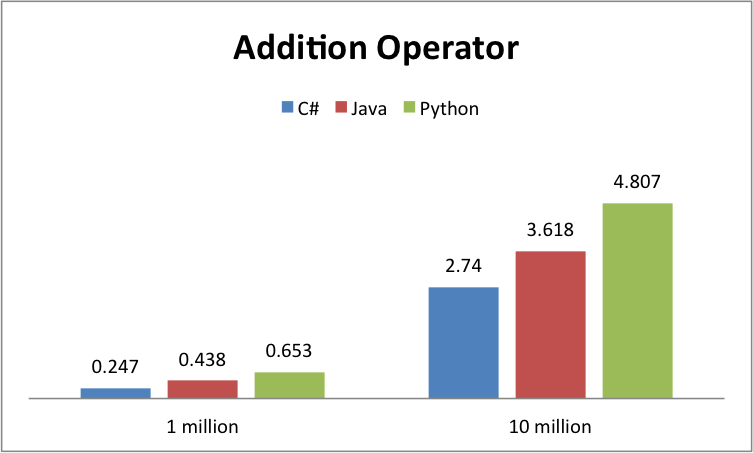
\includegraphics[width=0.48\textwidth]{chapters/media/addition.png}
		\label{fig:addition}
	}
	\subfigure[Test results from subtraction operator.]{
		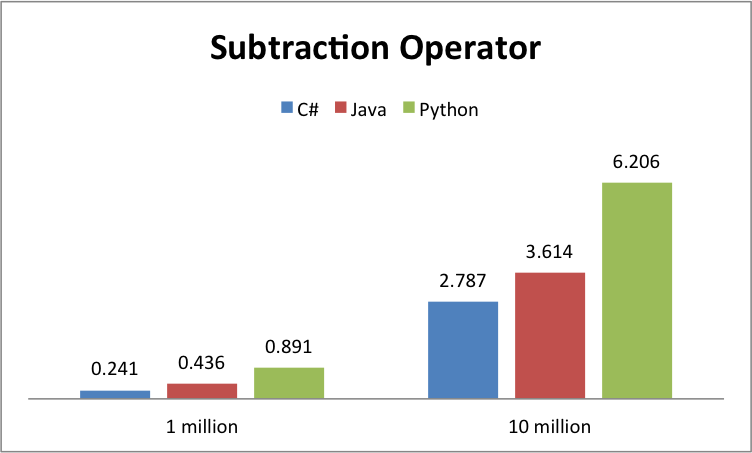
\includegraphics[width=0.48\textwidth]{chapters/media/subtraction.png}
		\label{fig:subtraction}
	}
}
\caption{Test results for the addition operator to the left and subtraction to the right.}
\label{fig:addition_subtraction}
\end{figure}

\begin{figure}[h]
\centering
\mbox{
	\subfigure[Test results from multiplication operator.]{
		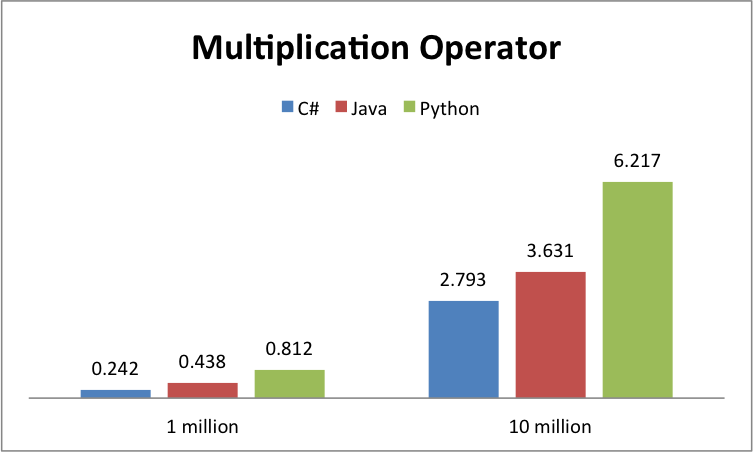
\includegraphics[width=0.48\textwidth]{chapters/media/multiplication.png}
		\label{fig:multiplication}
	}
	\subfigure[Test results from division operator.]{
		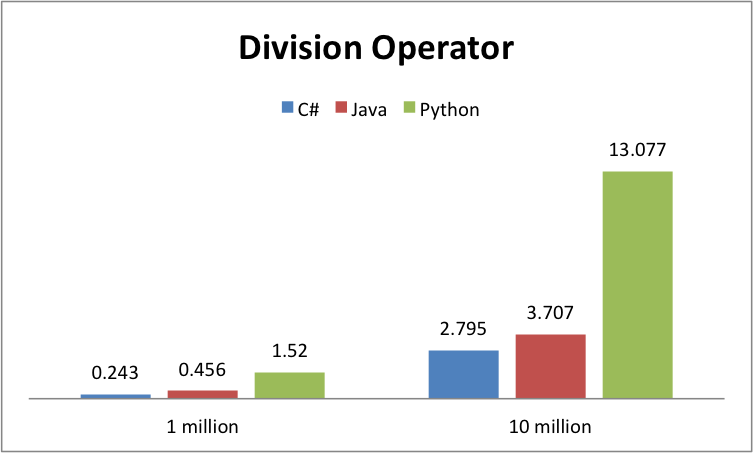
\includegraphics[width=0.48\textwidth]{chapters/media/division.png}
		\label{fig:division}
	}
}
\caption{Test results for the multiplication operator on the left and division to the right.}
\label{fig:multiplication_division}
\end{figure}

\begin{figure}[h]
	\centering
	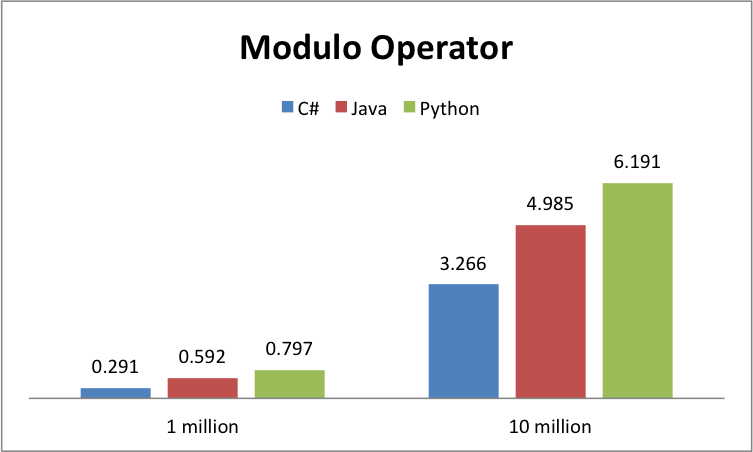
\includegraphics[width=0.48\linewidth]{chapters/media/modulo.png}
	\caption{Test results from modulo operator.}
	\label{fig:modulo}
\end{figure}

As can bee seen in Figure \ref{fig:addition_subtraction} - \ref{fig:modulo} the time complexity is linear, it takes about 10 times longer to operate on 10 million numbers compared with 1 million.  
